\section{Support Vector Machine}
\begin{figure}[htbp]
\centering
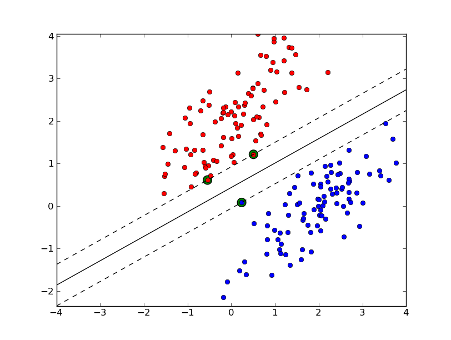
\includegraphics[width=3.0in]{image/SVM.png}
\caption{Finding the maximum gap hyperplane in SVM algorithm}
\label{SVM}
\end{figure}

Machining learning algorithms range from original K-means, Latent Dirichlet Allocation\cite{blei2003latent} to more complex ones such as Support Vector Machine, Neural Networks and Random Forest\cite{liaw2002classification}. These algorithms deal with classification or regression problems of all kinds. When choosing an algorithm to apply to a specific problem, we need to take a certain factors into consideration. Time complexity is one of the most limiting factors. When learning a large scale dataset, we often face the problem of runtime limitation. Support Vector Machine(SVM) is an important algorithm universally used is classification. It has high performance when working on certain training data and is good for simplifying polynomial problem into linear problem. In SVM algorithm, the computation time depends on large scale kernel matrix. Lots of effort have been made to optimize the runtime of SVM models.

One effective way is to reduce the number of selected features, called feature selection. Usually within a dataset there is only part of the data that we need to complete a classification. Many features are not that important in the final result and do not count for the classification. We only need to manually pick up the dependent ones regardless of the others which may take up a lot of space. This is a basic approach to reduce feature vector size\cite{weston2000feature}.
However, there may be sometime that we do not know if one feature weights over another and can not manually omit some of the features, or the feature numbers are large so selection can be lots of work. Feature subsets can then solve the problem by applying various algorithm. The most widely used algorithms are information gain\cite{kullback1951information}, 
, Gini\cite{yitzhaki1979relative}
 and correlation based feature selection\cite{hall1999correlation}.

Aside of modifying the dataset, we can also reduce time of I/O operations caused by communication. Within an iteration of SVM computation, the information of each round needs to be updated and therefore caused read and write operations. Harp is a plugin to Hadoop which specifically deal with this problem.

